\documentclass[11pt,a4paper]{article}
\usepackage[margin=0.9in]{geometry}
\usepackage{amsmath,amssymb,amsthm,booktabs,graphicx,enumitem,xr,float}
\usepackage[hidelinks]{hyperref}
\externaldocument{main}
% Generated from results.json; do not hand edit.
\newcommand{\TauMean}{18.052}
\newcommand{\TauSD}{1.006}
\newcommand{\TauTheory}{0.995}
\newcommand{\GammaMean}{0.346}
\newcommand{\AlphaMean}{0.798}
\newcommand{\GammaSD}{0.078}
\newcommand{\AlphaSD}{0.050}
\newcommand{\ChiMean}{0.5994}
\newcommand{\ChiSD}{0.0137}
\newcommand{\NoisyChi}{0.3356}
\newcommand{\NormalCoverage}{94.85\%}
\newcommand{\TCoverage}{95.00\%}
\newcommand{\NoisyCoverage}{2.35\%}
\newcommand{\BootCoverage}{95.00\%}
\newcommand{\BootCount}{57}
\newcommand{\RobustWindow}{0.737}
\newcommand{\PossibleWindow}{0.953}
\newcommand{\ChirpMean}{18.211}
\newcommand{\ChirpSD}{1.511}
\newcommand{\CleanMixRMSE}{0.029}
\newcommand{\MixedRMSE}{0.567}
\newcommand{\MSEAdd}{0.0019065}
\newcommand{\MSEInstant}{0.0020171}
\newcommand{\MSEExcluded}{0.0020625}
\newcommand{\MSEDelay}{0.0004147}
\newcommand{\MSEInclusive}{0.0004183}
\newcommand{\CleanTenRmse}{0.062}
\newcommand{\CleanTenKappa}{1.958}
\newcommand{\MixZeroRmse}{0.355}
\newcommand{\MixZeroKappa}{3.135}
\newcommand{\DriveZeroRmse}{0.332}
\newcommand{\DriveZeroKappa}{2.833}
\newcommand{\MixdriveZeroRmse}{0.557}
\newcommand{\MixdriveZeroKappa}{4.833}
\newcommand{\FalseConst}{20}
\newcommand{\FalseFourier}{0}
\newcommand{\AltGate}{0.07602}
\newcommand{\AltConst}{0.08154}
\newcommand{\AltFourier}{0.04252}

\setlength{\emergencystretch}{2em}
\newtheorem{proposition}{Supplementary Proposition}
\DeclareMathOperator{\im}{im}\DeclareMathOperator{\rank}{rank}
\title{Supplementary Methods and Verification\\\large Phase-Gated Interregional Transfer: Identifiability, Projection, and Completion Latency}
\author{Karem Abdelgalil}\date{6 October 2026}
\begin{document}\renewcommand{\thefigure}{S\arabic{figure}}\maketitle
\section*{S1. Reproduction contract}
Run \texttt{python -m pip install -r requirements.txt}, then \texttt{python reproduce.py}. The driver regenerates every revised analysis and all eleven revised figure files, including the conceptual roadmap, worked learning example, and reciprocal feedback checks, runs the independent verification script and builds manuscript macros from the generated numerical outputs. Python 3.12.14, NumPy 2.3.5, SciPy 1.17.0 and Matplotlib 3.10.8 were used. Figure PDFs can differ bytewise across metadata or platforms; numerical outputs and tolerances are the relevant reproducibility target.

The manuscript is compiled using \texttt{pdflatex main}, \texttt{bibtex main}, and two further \texttt{pdflatex main} runs. Compile this supplement and the response letter twice after the manuscript. The source archive contains compiled PDFs, full source, per-realization outputs and a checksummed manifest. The author supplies the public repository and project DOI listed in the main article. Archive-to-revision correspondence could not be independently verified; use the accompanying package for the numerical checks described here.

The \texttt{legacy\_supplied} folder preserves the user's original simulation, verifier, JSON, macros, selected figures and response letter. Its original simulation is rerun separately; its source-mixing results are retained in the main text and explicitly labeled as supplied-model checks. File names with parentheses identify the supplied originals. \texttt{legacy\_supplied/results.json} is the newly regenerated legacy output. A historical claim without an implementation is not silently promoted to a reproduced result.

\begin{table}[htbp]\centering\small
\caption{Executed revised analyses and independent random streams.}
\begin{tabular}{@{}p{.32\linewidth}p{.2\linewidth}p{.38\linewidth}@{}}\toprule
Analysis & Seed & Replication unit\\\midrule
Joint phase--gain recovery & 8102026 & 300 realizations; 32 phase trials/band; 48 gain samples\\
Coupling intervals and feature noise & 9102026 & 2000 realizations; 500 independent trials each\\
Pairs bootstrap & 9102027 & First 60 coupling realizations; 2000 resamples each\\
Delayed readout & 4026 & One 900-sample time series\\
Known chirp recovery & 10102026 & 300 realizations; 128 phase observations each\\
Signal-level mixing & 11102026 & 2000 independent complex observations\\
Independent algebraic verification & 20261005 & Randomized maps and fidelity bounds\\\bottomrule
\end{tabular}\end{table}

\section*{S2. Phase and gain observation details}
The revised manuscript, model functions, simulation, and figure labels all use $\alpha$ for receptive center, $\gamma$ for transfer phase, and $\tau$ for delay; $\eta=\alpha+\Omega\tau$ is the gate offset. The noiseless complex observation is
\[
 m(\psi)=a e^{\kappa(\cos(\psi-\alpha-\Omega\tau)-1)}e^{-i(\gamma+\Omega\tau)}.
\]
For component noise variance $s^2$, independent complex observations have information $I_{ab}=s^{-2}\operatorname{Re}\sum_q(\partial_a m_q)^*\partial_b m_q$. This convention removes the common factor-of-two ambiguity in complex-normal notation. Let $g'=dg/d\delta$ and $p=\gamma+\Omega\tau$. The derivatives are
\[
 \partial_\gamma m=-im,\quad
 \partial_\alpha m=-a g'e^{-ip},\quad
 \partial_\tau m=-\Omega a g'e^{-ip}-i\Omega m.
\]
Their combination $\Omega\partial_\gamma m+\Omega\partial_\alpha m-\partial_\tau m$ is zero. Amplitude derivatives do not break the ridge because they depend on the same gain-offset combination. A gain scan with $\kappa>0$ and nonzero amplitude must sample an informative range; measurements only at the peak have zero center derivative. Unknown arbitrary gain functions or nonstationary preferences are different models.

The implemented recovery separates observation channels: unwrapped phase observations are independent Gaussian errors of SD 0.2 rad around $\gamma+\Omega\tau$. There are 32 per band at 8 and 16 Hz. Their means give $\widehat\tau=(\bar\xi_2-\bar\xi_1)/(\Omega_2-\Omega_1)$ and $\widehat\gamma=\bar\xi_1-\Omega_1\widehat\tau$. The gain scan uses 48 evenly spaced $\psi$ values over one cycle, mean $0.9g(\psi-\eta)$ with $\kappa=2$, and independent noise SD 0.02. Least squares fits its center and nonnegative amplitude, initialized at the observed maximum, using a local center interval of width $2\pi$ and amplitude bounds $[0,2]$. The inferred $\alpha$ is wrapped to $(-\pi,\pi]$. Neither $\gamma$ nor $\alpha$ is forced equal to the other.

This Gaussian phase approximation is an additional calibrated observation model, not an exact assertion that arbitrary noisy cross-spectral angles are Gaussian. No discrete phase branch is recovered here. For the chosen frequencies, phase observations permit delay aliases separated by 125 ms without additional phase-branch information. A physiologically motivated bound, broadband onset measurement or a justified unwrapping rule must establish the branch before interpretation.

For fixed total weight and frequencies in $[L,U]$, the inequality $E[(\Omega-L)(U-\Omega)]\ge0$ gives $\operatorname{Var}(\Omega)\le(E\Omega-L)(U-E\Omega)\le(U-L)^2/4$. Equal mass at the endpoints attains the bound. This supplies an optional design refinement under fixed noise and transfer-phase assumptions.

For equal per-trial phase variance $0.2^2$ and 32 trials, the variance of a frequency's mean is $v=0.2^2/32$. Predicted delay SD is $\sqrt{2v}/[2\pi(16-8)]=\TauTheory{}$ ms, compared with \TauSD{} ms observed. This tests the conditional linear estimator, not the biological validity of a frequency-independent transfer phase.

A known chirp with $\theta(t)=\Omega_0t+ct^2/2$ gives unwrapped phase observation $Y=\gamma+\theta(t)-\theta(t-\tau)+e$. Its slope is $c\tau$ and its intercept is $\gamma+\Omega_0\tau-c\tau^2/2$. The script uses $c=40$ rad/s$^2$, 128 equally spaced times in $[0,1]$, and independent SD 0.2 rad over 300 realizations. The resulting delay mean/SD are \ChirpMean{}/\ChirpSD{} ms. This example has different sample counts and excitation from the historical chirp claim; it is not a reconstruction of the old figure.

\section*{S3. Effective bilinear subspace theorem}
Let $M_1$ and $M_2$ map two independently controllable content spaces into a common receiver space $\mathbb R^n$. Set $S_i=\im M_i$, $S=S_1+S_2$, with dimensions $r_i=\dim S_i$. Select orthonormal bases $p_1,\ldots,p_{r_1}$ and $q_1,\ldots,q_{r_2}$, and a fixed bilinear map $B:\mathbb R^n\times\mathbb R^n\to\mathbb R^n$. Form
\[
 C_B=[B(p_1,q_1)\ \cdots\ B(p_a,q_b)\ \cdots\ B(p_{r_1},q_{r_2})],
 \qquad A=[M_1\ M_2].
\]
\begin{proposition}[Interaction-generated subspace]
For independently variable inputs and a nonzero fixed interaction coefficient, the linear span of reachable mean outputs of $y=u+v+\chi B(u,v)$ is
\[
 W=S+\operatorname{span}\{B(p_a,q_b)\}.
\]
The number of extra linearly independent receiver directions is
\[
 d_B=\rank[A\ C_B]-\rank A=\rank(QC_B)
 \le\min(n-\dim S,r_1r_2),
\]
where $Q$ is orthogonal projection onto $S^\perp$. If factorial scaling is available with $H\ne L$, complement factorial contrasts spanning the basis pairs identify the effective span $\im(QC_B)$, although not the anatomical locus of $B$.
\end{proposition}
\begin{proof}
Let $L$ be the linear span of all possible outputs and let $W=S+\im C_B$. Express $u=\sum_a x_ap_a$ and $v=\sum_b y_bq_b$. Bilinearity gives $B(u,v)=\sum_{a,b}x_ay_bB(p_a,q_b)$, so every output lies in $W$ and $L\subseteq W$.

For the reverse inclusion, unrestricted independent inputs include $(u,0)$, $(0,v)$, and $(0,0)$. Their outputs are $u$, $v$, and zero, so $S\subseteq L$. Subtract the two single-input outputs from a joint output:
\[
y(u,v)-y(u,0)-y(0,v)=\chi B(u,v).
\]
This difference belongs to $L$, which is a linear space. Since $\chi\ne0$, each basis-product vector $B(p_a,q_b)$ belongs to $L$. Therefore $\im C_B\subseteq L$ and $W\subseteq L$, proving equality.

The columns of $[A\ C_B]$ span $W$, while those of $A$ span $S$. The restriction of $Q$ to $W$ has kernel $S$: a vector in $W$ is killed exactly when it lies in $S$. Its image is $\im(QC_B)$, because $Q$ kills $A$ and every remaining column is a projected product. Rank--nullity on $W$ therefore yields $\dim W-\dim S=\rank(QC_B)$, establishing both rank equalities. The projected products lie in the $(n-\dim S)$-dimensional complement and are spanned by $r_1r_2$ columns, proving the upper bound.

Finally, the main-text factorial-contrast proposition applied to each basis pair and followed by $Q$ gives $\chi(H-L)^2QB(p_a,q_b)$. For $H\ne L$ this is a common nonzero scalar multiple of each projected product. Their span equals $\im(QC_B)$, regardless of the value of that nonzero scalar. This identifies an effective output span across conditions, not each vector's attainability in a single condition or the location of the nonlinearity.
\end{proof}
This is a statement about the span of multiple possible outputs, not a claim that every vector in $W$ is achievable by one input pair. Restricted content co-variation, null gains, saturation, uncalibrated $Q$, or an unknown nonlinear sensor map invalidate its experimental identification conditions. The rank bound is elementary multilinear algebra. Its use here is to specify what an interaction would add beyond additive translated content, not to introduce a universal generative theory of ideas.

In the coded example, $S_1=\operatorname{span}(e_1)$, $S_2=\operatorname{span}(e_2)$, and $B(u,v)=u_1v_2e_3$. Additive rank is two and augmented rank is three. The third coordinate is $0.6ab$, with nonzero factorial response but no additive contribution. A joint readout nonlinearity gives the same effective response, so causal localization needs additional recordings/interventions.

\subsection*{Finite interaction memory}
For pathway outputs that already include conduction and local processing, define
\[
 I(t)=\chi\int_0^\infty\!\int_0^\infty k(s,q)B(U(t-s),V(t-q))\,ds\,dq.
\]
Here $k$ is a scalar integrable memory kernel (not a vector-valued expression mixed into its own definition). Independent constant scalings commute with this bilinear integral; the same factorial identity holds with $B(U,V)$ replaced by the integral. Its complement remains in the effective bilinear span. The kernel can have signed effects and cancellations, so two nonzero inputs are necessary for this term but not sufficient for a nonzero output. Multiple memories and joint readouts can be observationally equivalent. $B$ and $k$ are not separately recovered by the contrast; even their scalar normalization can be exchanged.

\begin{figure}[htbp]\centering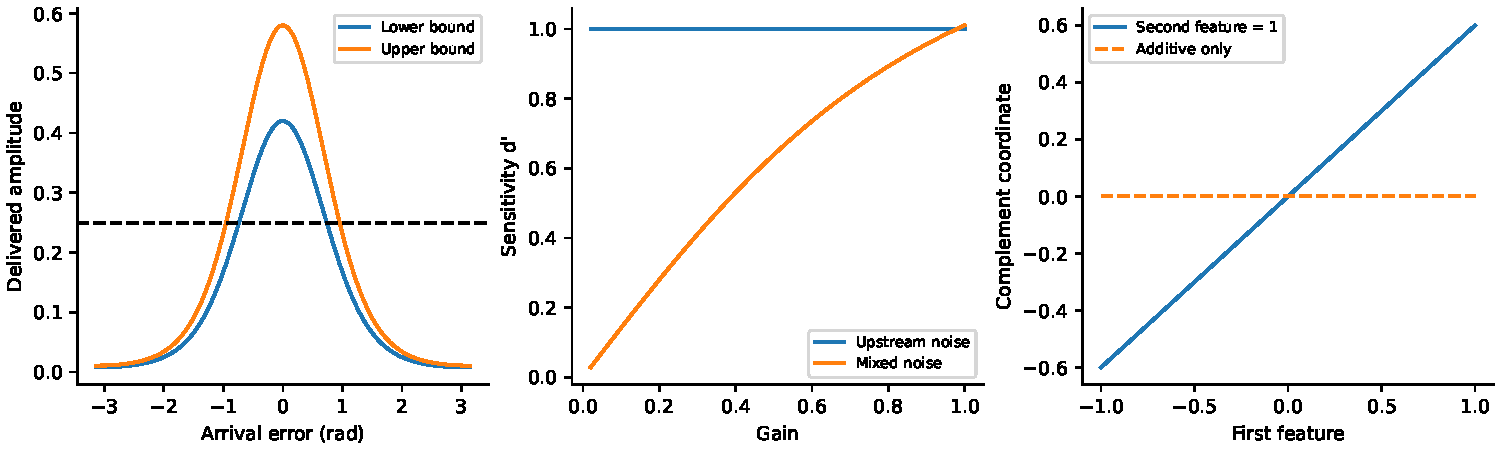
\includegraphics[width=\linewidth]{figure_delivery.pdf}
\caption{S1. Uncertainty-aware delivery, conditional sensitivity, and a receiver coordinate generated by the stipulated interaction. The positive exponential gate never closes exactly.}\end{figure}

\section*{S4. Delivery, sensitivity and falsification checks}
The exact gate threshold uses the calibrated item's $A_v=|v^\top Mz|$, not mere membership of $v$ in a pathway image. For instance $M=\operatorname{diag}(1,0)$, $v=e_1$ and $z=e_2$ give zero projection even though $v\in\im M$. For $A_v<\vartheta$, no phase reaches threshold. In the robust example $\widehat A_v=0.5$ and uncertainty 0.08 yield lower/upper amplitudes 0.42/0.58. With threshold 0.25 and $\kappa=2$, the lower bound passes only inside \RobustWindow{} rad; delivery is merely possible inside \PossibleWindow{} rad. Outside the latter interval it is certified below threshold.

A proposed Gaussian sensitivity likelihood distinguishes signal, upstream noise and downstream noise. For positive downstream noise the gain derivative in Eq.~\ref{eq:sensitivity} is positive; pure upstream noise yields constant $d'$ at positive gain and a degenerate case at zero gain. This follows from the observation model, not from geometric feasibility. A monotone saturated function $f(rC)=\tanh(rC)$ gives
\[
 \frac{\partial^2 f}{\partial r\partial C}
 =\operatorname{sech}^2(z)[1-2z\tanh z],\qquad z=rC.
\]
At $z=2$ this is approximately $-0.202$, so monotonicity is insufficient for a universal positive interaction coefficient. Verification includes this counterexample rather than a circular ``corollary passed'' assertion. The confirmatory choice-likelihood study is not simulated in this package.

\section*{S5. Coupling coverage and bootstrap implementation}
For each of 2000 independent realizations, sample $u,v$ independently uniform on $[-1,1]$, phases independently uniform on $[-\pi,\pi]$, and set $a=g(\delta_1)u$, $b=g(\delta_2)v$. The true model is
\[
 y=0.2+0.7a+0.4b+0.6ab+e,\quad e\sim N(0,0.02^2),\quad n=500.
\]
OLS fits $X=(1,a,b,ab)$ using least squares, and covariance is $\widehat s^2(X^\top X)^{-1}$, with residual variance divided by $500-4$. The design is full rank almost surely. Conditioning on $X$, independent homoscedastic Gaussian errors give exact Student-$t$ pivots. Correlation among regressors affects the covariance already represented by the matrix inverse; it does not create an omitted variance term. Normal intervals use 1.96; Student-$t$ intervals use its 0.975 quantile at 496 degrees of freedom. Per-run standard errors and both endpoints are stored.

The observed Student-$t$ coverage is \TCoverage{} (1900/2000). Its Monte Carlo Wilson interval is approximately $[93.96\%,95.87\%]$. The noisy-feature experiment adds independent Gaussian SD 0.15 noise directly to $a$ and $b$, fits the same formula to those noisy inputs, and stores all estimates/intervals. It gives \NoisyCoverage{} (47/2000), with Monte Carlo interval approximately $[1.77\%,3.11\%]$ and mean coefficient \NoisyChi{}. These results demonstrate conditional failure under this specified feature-error mechanism. They do not establish that all feature-noise placements yield the same attenuation or coverage.

For the first 60 new realizations, independently resample whole trial pairs with replacement 2000 times and refit all four coefficients. Percentile endpoints are the 0.025 and 0.975 quantiles. A multinomial-count implementation computes weighted sufficient statistics in batches of 100; it is equivalent to drawing trial indices for independent pairs. No time-series or participant block is resampled here. Bootstrap coverage is \BootCount{}/60 and the Monte Carlo interval is approximately $[86.3\%,98.3\%]$. The same first 60 Student-$t$ and normal intervals also cover in 57/60. Neither small-sample comparison supports replacing exact conditional Student-$t$ inference with a generic bootstrap recommendation.

The historical supplied exact-feature run covered 52/60. Under true 95\% coverage, the lower-tail probability of 52 or fewer successes is about 0.00979. Preserve that outcome and investigate its Monte Carlo behavior without asserting a diagnosed systematic cause. The new exact-feature run is compatible with nominal coverage; it is a separately specified diagnostic with a new seed, not an overwritten historical result. Historical noisy-feature and excluded-product summary values lacked corresponding code and are superseded by the explicitly implemented analyses above.

\section*{S6. Temporal readout settings}
The seeded 900-sample signal has 5 ms sampling. Two independent Gaussian content coordinates are smoothed with a five-sample moving average. Encoding $D_j=\left(\begin{smallmatrix}1&.3\\.2&1\end{smallmatrix}\right)$, target $D_i=\left(\begin{smallmatrix}.8&-.2\\.1&1.1\end{smallmatrix}\right)$ and exact $T=D_iD_j^{-1}$ are supplied. The first translated signal uses conduction three samples and processing delays two/four samples with weights 0.6/0.4. The second has four-sample total delay. Time-varying gains are sinusoidal with known values; the interaction uses two/six extra samples and coefficient 0.6. Independent output noise has SD 0.02.

After a 30-sample burn-in, train/validation/test segments have 500/150/220 samples. Interaction lags are searched over integers 0--8 using validation MSE only. Fits on train plus validation are then evaluated on untouched test responses. Predictor histories are available, but no test response enters fitting or lag selection. Symmetric smoothing defines the synthetic latent stimulus, not a decoder trained on future test responses.

Feature columns are explicitly: additive $(1,a,b)$; instantaneous $(1,a,b,ab)$; quadratic excluded $(1,a,b,ab,a^2,b^2)$; delayed $(1,a,b,a_{t-l_p}b_{t-l_c})$; quadratic inclusive adds $a^2,b^2$ to the delayed model. The excluded comparator excludes the selected delayed product but includes the instantaneous product. Its regenerated MSE is \MSEExcluded{}, not the old 0.00052 assertion. Inclusive quadratic MSE \MSEInclusive{} closely matches delayed \MSEDelay{} and illustrates flexible predictive equivalence.

\begin{figure}[htbp]\centering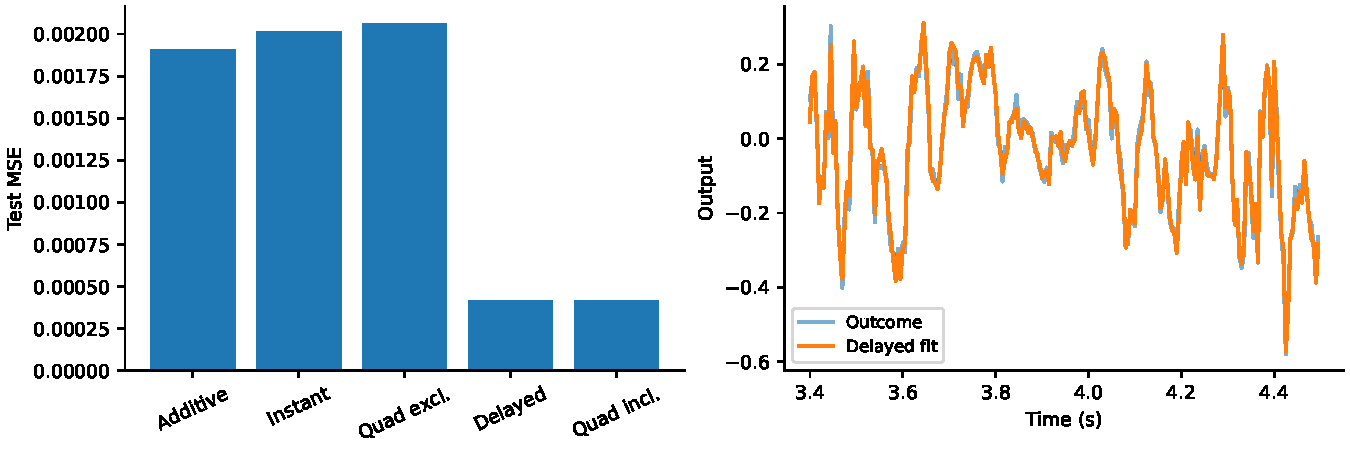
\includegraphics[width=\linewidth]{figure_temporal.pdf}
\caption{S2. Conditional temporal prediction with both excluded and inclusive quadratic competitors. One synthetic realization; maps, input histories and gains supplied.}\end{figure}

\section*{S7. Complex signal mixing}
To avoid treating angles as additive voltages, the illustration forms complex signals $x=1+e_x$, $y=e^{-i(\gamma+\Omega\tau)}+e_y$, with independent real/imaginary error SD 0.02, then adds a shared complex component $c=e^{0.7i}$ with weights 0.3 and 0.7. Observed phases are $\arg(yx^*)$ and $\arg[(y+0.7c)(x+0.3c)^*]$. RMSE against the true transfer phase is \CleanMixRMSE{} and \MixedRMSE{} rad. This is a signal-level contamination example. It does not prove identifiability preservation for arbitrary common-drive generators or provide an EEG/MEG lead-field model. No harmonic distortion is claimed from an ideal filter that removes that harmonic.
\begin{figure}[H]\centering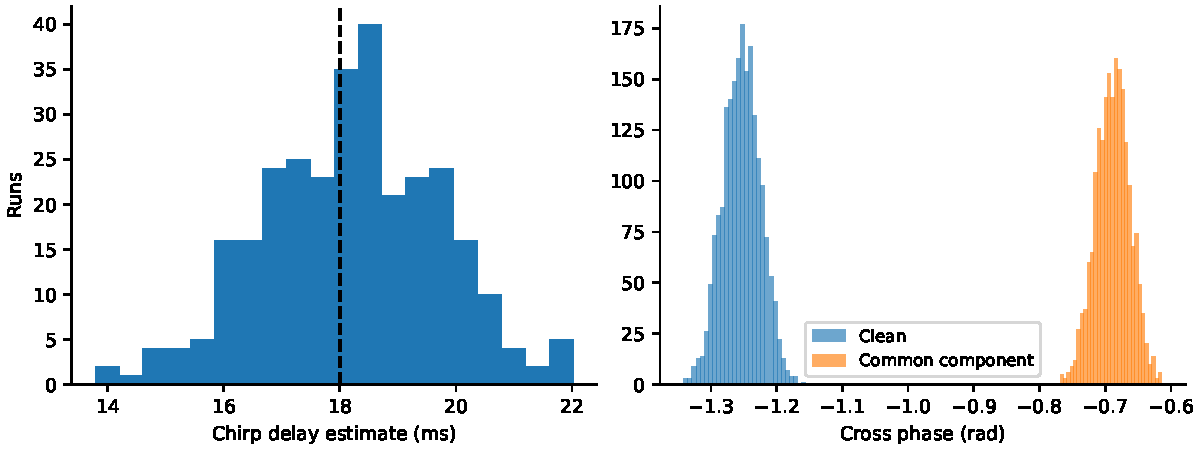
\includegraphics[width=.95\linewidth]{figure_escape_mixing.pdf}
\caption{S3. Known-chirp recovery and phase distortion under a shared complex signal component. Both are synthetic and use separate fixed seeds.}\end{figure}

\section*{S8. Verification and retained learning postulate}
\texttt{verify.py} independently checks ridge likelihood equivalence, Fisher null directions by numerical differentiation, two- versus one-frequency rank, harmonic-scaled ambiguity, weighted-information determinants, translation factorization and impossibility, randomized fidelity bounds, exact threshold feasibility, map-uncertainty bounds, the bilinear complement rank and factorial identity, a sensitivity counterexample, transient-onset non-equivalence, and recomputed coverage counts from individual endpoints. It writes an explicit check record. Algebra checks are not used as evidence for a unique neural generator.

The historical learning update $T_{n+1}=T_n+\epsilon\ell_n r_n(v_n-T_nu_n)u_n^\top$ is retained in the legacy material, not a primary claim. A fixed pair contracts its residual if $0<\epsilon\ell r\|u\|^2<2$. A zero opportunity flag forces a frozen trace by construction. Activity-only learning and ungated turnover would be required empirical rivals; this imposed split is not independent evidence of plasticity biology.
\section*{S9. Retained source-mixing checks and coverage provenance}
Run the supplied simulation in its own directory with \texttt{python legacy\_supplied/simulate.py} through the reproduction driver, which sets that directory as the working directory. It generates seven legacy figures and \texttt{legacy\_supplied/results.json}. These include the original marker, order, trace, serial-path, coupling, delayed readout, and 8 Hz source-mixing checks. The original verifier is rerun against those outputs. Original reporting macros and response text are retained as provenance; the revised manuscript does not rely on their unsupported causal explanations.

For the retained sensor model, sampling is 250 Hz and an ideal 6--10 Hz filter removes the imposed 16 Hz harmonic. Fitted concentration is a descriptive regression result under this pipeline. A removed harmonic does not test robustness to harmonic contamination retained in the observation band. The original 52/60 coverage result is recorded as historical; the revised 2,000-run experiment uses an explicit correct Gaussian regression model, and its 60-run bootstrap subset refits every coefficient on each resample.

\begin{figure}[htbp]\centering\includegraphics[width=.92\linewidth]{legacy_supplied/figure6.pdf}\caption{S4. Retained supplied sensor simulation: stylized source mixing, common drive, and fitted gate behavior under the ideal 6--10 Hz filter. This is a recovery diagnostic, not a lead-field or neural validation.}\end{figure}
\section*{S10. Projection communication and completion checks}
Theorem~\ref{thm:inter} uses a signed receiver contribution $q=g(\delta)v^\top Mz$. For fixed phase, map, and other inputs, the exact source-content contrast is $q(z+\epsilon d)-q(z)=\epsilon g(\delta)v^\top Md$. Independent randomized checks evaluate this identity on maps, items, readout directions, contrast directions, and phase values, including $\pi$. They distinguish a structurally supported readout from an item whose readout projection vanishes. The regional interpretation requires that these modeled variables and maps correspond to independently calibrated brain measurements.

For nonnegative normalized processing kernels, a same-sign projection bounded away from zero prevents cancellation. The verifier checks a weighted discrete kernel realization and a separate counterexample with equal positive and negative projections, whose integral is zero despite nonzero pointwise projections. Neither a carrier ridge nor structural support removes this temporal issue.

The instantaneous completion result applies after content is available at the receiver. Use the full transfer convolution for nontrivial processing memory. A nonzero supported item may never cross a positive threshold. Nonzero gain at $\pi$, readout directions outside the image with nonzero projection, supported readouts with a null item, and compensated carrier phase with shifted transient onset are independently checked in \texttt{verify.py}. A gain intervention need not identify the physical delay to test its amplitude consequence. A scalar route aggregate cannot replace channel gain without calibration.

The supplied main paper's stronger assertions---finite lag from support alone, necessary alignment of both gates for every bilinear output, and a positive global linear interaction from monotonicity alone---are not consequences of the model. The revision replaces them by exact feasibility, an explicit first-passage definition, and derivatives under a specified Gaussian behavioral model.
\section*{S11. Proof conventions and regularity conditions}
Main-text proofs now give constructions, norm estimates, score-factorization arguments, and both directions of the relevant equivalences. Norms are Euclidean and induced operator norms unless a Frobenius norm is explicitly indicated. Parameter-rank claims are local on calibrated unwrapped branches. The delivery-window inversion assumes positive $\kappa$; the zero-concentration case is handled separately. First-attainment claims assume a continuous gate trajectory; this avoids equating a nonattained infimum with an actual event. Expected learning assumes integrability of the initial translation and the weighted excitation matrix. These clarifications do not turn conditional model results into empirical validation.

\section*{S12. Integrated results and additional verification}
The main text now contains the effective bilinear rank result of Supplement S3, the communication-under-map-uncertainty bound, and a gain-weighted learning proposition. The uncertainty bound is checked using admissible operator-norm perturbations. Interaction rank is checked on 100 independently generated content maps and bilinear coefficient tensors: the rank increment equals the complement-product rank and respects the dimension bound. Expected learning is checked by enumerating a finite independent teaching-pair distribution and comparing each averaged update to Eq.~\ref{eq:meanlearning}; the test also verifies that an unexcited direction remains unchanged. These are algebraic operating-condition checks, not new neural datasets.

The repository and DOI are included as author-supplied project identifiers. The browser lookup could not retrieve their current contents, so no statement that the cited archive contains this exact revised source is made. A local checksummed ZIP is supplied independently.
\section*{S13. Readability revision and notation contract}
The revised code uses the same parameter names as the main article. The \texttt{complex\_mean} arguments, in order, are \texttt{psi}, \texttt{O}, \texttt{gamma}, \texttt{alpha}, and \texttt{tau}. Here \texttt{psi} is the calibrated simultaneous probe phase, \texttt{O} is angular frequency, and \texttt{gamma}, \texttt{alpha}, and \texttt{tau} are respectively transfer phase, receptive center, and conduction delay. The joint-recovery vectors are stored in that parameter order. Regression interaction coefficients such as $\beta_{CR}$ are different symbols and are not receptive centers. Original supplied files under \texttt{legacy\_supplied} are preserved without notation migration.

The exact worked learning example uses two coordinates, gain $1/2$, step size 0.4, and $T_*=I_2$. Restricted teaching has $G=\operatorname{diag}(1/2,0)$; equal-probability teaching on both signed coordinate directions has $G=I_2/4$. The independent verifier enumerates both input distributions and checks the closed-form mean matrix, the unchanged unexcited column, and the two column-error curves. \texttt{make\_reader\_figures.py} generates the diagram and the exact curves; no neural learning data are used.

The source and rendered sensitivity equation use distinct upstream and downstream noises, $\varepsilon_u$ and $\varepsilon_d$. The readability revision labels them explicitly and preserves their independence assumption. The proposed behavioral readout is not automatically a Gaussian readout of the bilinear output: that substitution would require a new noise model.
\section*{S14. Reciprocal transfer and latency: complete reproduction specification}
\texttt{simulate\_reciprocal.py} generates \texttt{reciprocal\_results.json} and \texttt{figure\_reciprocal.pdf}. These are constructed model examples, not fitted estimates. The source uses seconds throughout, with milliseconds only on figure axes. The step input begins at time zero; all previous content is zero. Fixed gates and pathway weights are absorbed into the real maps $L_{PQ},L_{QP}$. Processing is instantaneous in the time-domain theorem; unknown processing memory would require a different prediction. Positive $T_{\rm loop}$ ensures finitely many active terms at any finite time.

The scalar example uses $a=0.2$, $\beta=0.5$, $\tau_f=0.018$ s, $\tau_b=0.012$ s, and $\theta=0.34$. A time grid from 0 to 0.200 s has spacing 0.001 s; exact event times determine right-continuous steps rather than interpolated threshold estimates. Independently summing the geometric increments gives $0.2$ at 0.018 s, $0.3$ at 0.048 s, and $0.35$ at 0.078 s. The crossing has two returns. Removing feedback ($\beta=0$) yields no crossing at 0.34; a threshold of 0.4 is the original asymptotic limit and is not attained in finite time. These two null outcomes are stored as JSON \texttt{null} rather than invented finite lags. The code computes the minimum crossing index by summing plateaus, avoiding a logarithmic ceiling error at exact equality.

The zero-return example uses $L_{PQ}=\operatorname{diag}(0.5,0)$ and $L_{QP}=\operatorname{diag}(0,0.5)$ with item $d=e_1$. Its direct vector is $(0.5,0)^\top$ and its first returned vector is exactly zero. A separate verifier example uses $L_{PQ}=I_2/2$, $L_{QP}$ with off-diagonal entries $1/2$, $d=e_1$, and readout $v=e_2$: the first scalar contribution is zero but a later return is nonzero. Thus absence in a particular first readout is weaker than absence of the complete delivered vector. Neither counterexample assumes that the brain uses these maps.

The carrier comparison uses 8 Hz, $\kappa=2$, and edge tuples $(\gamma,\alpha,\tau,M,\psi)$ equal to $(0.25,0.8,0.018,0.55,0.9)$ and $(-0.1,0.6,0.012,0.5,0.7)$. Apply the ridge shifts $u_f=0.004$ s and $u_b=-0.002$ s on the two edges. The response $K_f/(1-K_fK_b)$ differs by approximately $8.9\times10^{-17}$, while the anchored first three opportunity times change from $(0.018,0.048,0.078)$ to $(0.014,0.042,0.070)$ s. The phase factors are stationary observation nuisances. These general-phase carrier examples do not assert that the real-map step response has that same unknown broadband phase realization; the time-domain echo theorem uses absent or calibrated instantaneous processing.

\paragraph{Independent verification.} With the verifier's fixed seed 20261005, 100 random map pairs have sizes $3\times2$ and $2\times3$, with each spectral norm rescaled to 0.6. Their product norm is at most 0.36. At each of 100 integer times, a direct two-population recurrence with forward delay three steps and reverse delay two steps is compared against the explicit matrix echo sum, using absolute tolerance $10^{-12}$. The verifier also checks all threshold regimes for amplitudes $0.1,0.2,0.7$ and loop gains $0,0.2,0.5,0.8$, including equality with the asymptotic limit. It checks 100 independently sampled pairs of carrier operators under compensated shifts, at tolerance $10^{-12}$. A signed-return counterexample rejects automatic monotonic improvement under unrestricted matrices. These are separate checks of equations and boundary cases, not tests that merely compare a function with itself.

\paragraph{Empirical discrimination and limits.} The isolated-loop prediction is that changing only the reverse map or gain changes later increments while preserving the initial forward increment. A rival with independent late inputs, joint readout nonlinearities, or changed sender activity could mimic or violate that prediction; those quantities require simultaneous measurement and intervention controls. A prefrontal/contralateral application additionally needs specific source populations, calibrated readouts, anatomical path validation, and independent latency measurements. Report status cannot be substituted for an experience measurement. Public code must include this exact revision before the archive correspondence statement can be strengthened.
\section*{S15. Operator limit, general returns, behavioral bridge, and MSE uncertainty}
The discrete-delay loop is the zero-processing-memory limit of the full retarded feedback architecture, not an unrelated second model. Unit point masses are interpreted as limits of normalized causal densities, with convergence on bounded continuous inputs and a uniform contraction bound. A step response at a discontinuity is not covered by pointwise continuity. The verifier compares a direct delayed recurrence with a two-tap forward processing kernel against the corresponding operator Neumann series; it separately checks the continuous-input approximate-identity limit.

Proposition~\ref{prop:generalpassage} uses general matrix partial sums and the tail error $E_m$, rather than scalar powers of an assumed invariant channel. One hundred random matrices of spectral norm 0.7 are checked for forty partial sums against the independent resolvent limit and the geometric error bound. A rotational example crosses 0.9 at the first contribution even though its eventual readout is 0.8. Equality with the limit has no general nonattainment implication. The finite Krylov support condition follows from Cayley--Hamilton. Signed and absolute thresholds are explicitly distinguished.

Corollary~\ref{cor:rank-sensitivity} supplies an explicit Gaussian bridge between interaction rank and decision sensitivity. Its positive-definite covariance is independently calibrated and held fixed; whitening and complement projection remove the additive class contrast. An innovation-only readout reaches $|\chi a_1a_2|\|Q_\Sigma\Sigma^{-1/2}b\|$. A class-independent product can have positive innovation rank and zero decision contrast. The verifier checks the squared-discriminability decomposition with nonisotropic covariance and the simultaneous-sign-reversal counterexample. This readout assumption does not follow from rank itself.

\paragraph{MSE comparison protocol.} \texttt{compare\_mse.py} reruns the complete delayed generator for 300 independent realizations at seed 402600. Each realization uses 900 samples, a 30-sample initial exclusion, 500 training samples, 150 validation samples, and 220 untouched test samples. Validation alone chooses a lag pair from $\{0,\ldots,8\}^2$; fitting on training plus validation then precedes test prediction. Four rivals and the delayed predictor share the same realization. The inferential unit is the complete realization, not individual temporally correlated test samples. All selected lags, model MSEs, paired differences, mean-difference intervals, raw tests, and Holm adjustments are stored in \texttt{mse\_comparison\_results.json}. The script generates the main-text table directly from those outputs.

For a rival's paired differences $D_j$, the pointwise interval is $\bar D\pm t_{0.975,299}\,s_D/\sqrt{300}$. Two-sided one-sample tests use those same paired differences, and Holm adjustment covers the four-rival family. These intervals quantify Monte Carlo mean-risk uncertainty under the specified synthetic generator. They are not simultaneous confidence intervals, temporal-sample intervals, practical-equivalence tests, or neural-data validation. The tiny inclusive-quadratic difference is statistically detectable; it is not described as exactly equal performance. The independent verifier recomputes means and confidence limits from all individual records.

\input{dataset_review/public_data_supplement.tex}
\setcounter{figure}{8}
\section*{S17. Stable non-normal returns, innovation geometry, and gate calibration}
Run \texttt{python strengthen.py} to regenerate Supplementary Figures S9--S10. Numerical output is saved in \texttt{strengthening\_\allowbreak results.json}. S9 uses the exact matrix, input and readout in Proposition~\ref{prop:stable-returns}. The Lyapunov matrix is computed by a discrete Lyapunov solver and independently checked against its defining identity. Exact partial sums and tail errors are compared with the norm certificate. The accompanying script also recomputes the minimum threshold index rather than inferring it from a plotted interpolation. The singular-value planning calculation checks the stated 179-trial illustration; it does not estimate biological variance.
\begin{figure}[H]\centering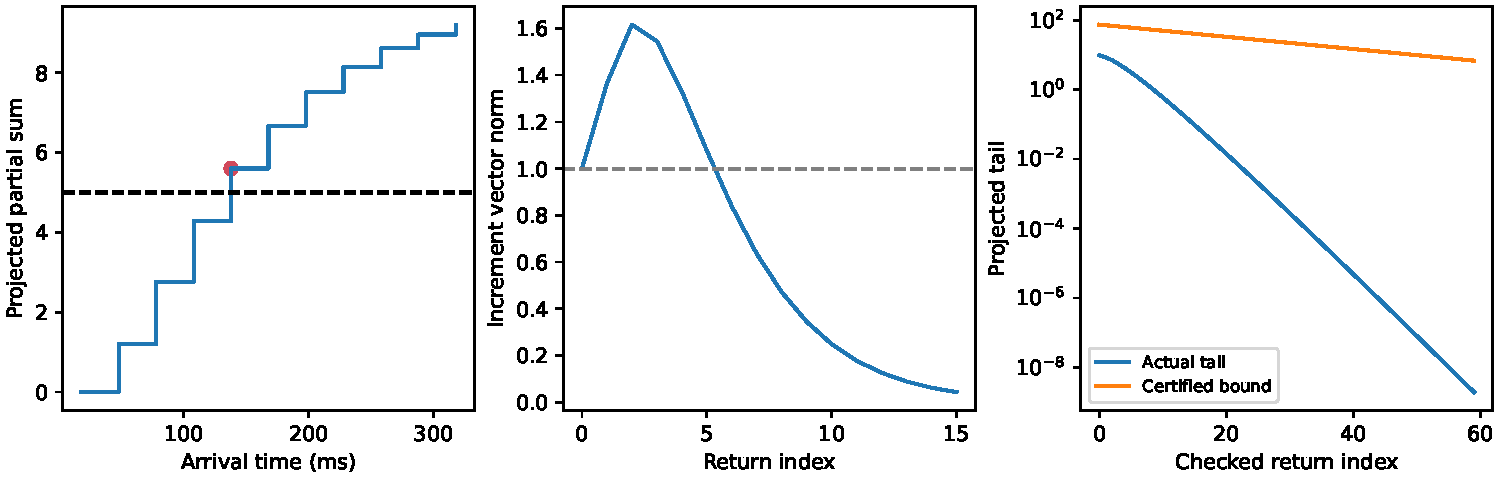
\includegraphics[width=.95\linewidth]{figure_nonnormal.pdf}\caption{Stable non-normal returns. Left: a zero direct readout crosses threshold 5 at the fourth return. Middle: individual increments can amplify in Euclidean norm although the spectral radius is 0.65. Right: the Lyapunov tail bound contains the actual projected tail and can be conservative. All values are synthetic.}\label{fig:supp-nonnormal}\end{figure}
\begin{figure}[H]\centering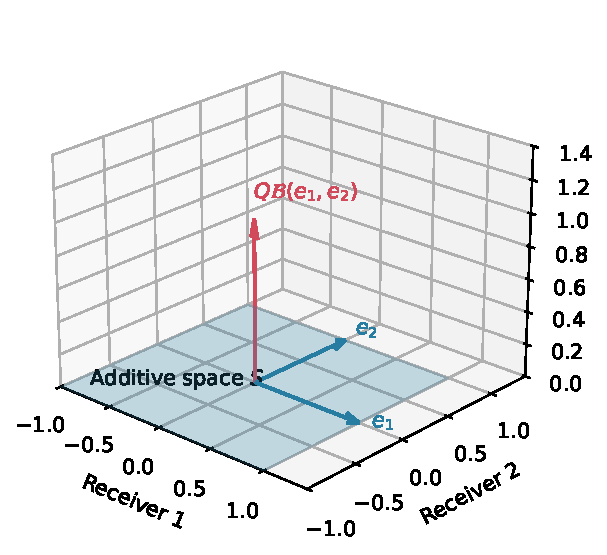
\includegraphics[width=.72\linewidth]{figure_innovation_geometry.pdf}\caption{Interaction geometry for the exact three-coordinate example: additive responses occupy $S=\operatorname{span}\{e_1,e_2\}$, while the bilinear product contributes along $e_3\in S^\perp$. The added rank is one across conditions; a class-independent product has zero class contrast despite this rank.}\end{figure}
For the gate $g(\delta)=\exp[-\kappa(1-\cos\delta)]$, $\kappa=0$ gives constant gain; finite positive $\kappa$ gives positive opposite-phase attenuation. A half-height angle exists when $\kappa\ge\log(2)/2$ and solves $\cos\delta_{1/2}=1-\log(2)/\kappa$. At smaller concentrations the gate stays above half height even at opposite phase. Estimate amplitude, center and concentration on independent calibration probes with matched input content, then freeze them. Unknown filter phase and upstream state changes can invalidate the biological interpretation. The example $\kappa=2$ is an illustrative concentration, not a measured universal neural value.

\section*{S18. Symbol glossary and model boundaries}
\begin{center}\small\begin{tabular}{@{}p{.25\linewidth}p{.67\linewidth}@{}}\toprule
Symbols & Meaning\\\midrule
$z,d,D_j,D_i,T_{ij},M$ & Anchored item; source perturbation; encoders; translation; composite translated encoder\\
$B_{ij}$ & Translation error $T_{ij}D_j-D_i$\\
$\Omega,\tau,\alpha,\gamma$ & Angular frequency; conduction; receptive center; carrier transfer phase\\
$\eta,\xi,\psi,\Delta$ & Gate offset; carrier offset; calibrated probe phase contrast; arrival error\\
$g,\kappa,r,w,H,h$ & Gate; concentration; gain; pathway weight; Fourier processing response; causal processing density\\
$a_v,A_v,\theta_{\rm comm}$ & Delivered item amplitude; its maximum over phase; operational threshold\\
$P,Q,L_{PQ},L_{QP}$ & Loop populations and forward/reverse content maps (first index is receiver)\\
$A,p_0,v,T_{\rm loop}$ & Return product; initial projected vector; readout; round-trip delay\\
$\mathcal S_d,z_m,E_m,G_A$ & Item Krylov space; scalar partial sum; tail bound; Lyapunov metric\\
$S_1,S_2,S,C_B,d_B$ & Pathway images; their sum; basis-product matrix; added innovation rank\\
$\mathcal B,k,\chi,U,V$ & Bilinear map; interaction memory; coefficient; translated inputs\\
$\Sigma,W,Q_\Sigma,\lambda$ & Readout covariance; whitening; complement projector; interaction gain\\
$T_n,T_*,u_n,v_n,G$ & Learned map; target; teaching input/target; weighted excitation\\
$\varepsilon,\ell_n,r_n$ & Learning step; opportunity flag; teaching gain\\\bottomrule
\end{tabular}\end{center}
Some symbols are local to distinct modules: $Q$ is a regional loop signal in the reciprocal model and an orthogonal projector in the interaction-rank proposition; $A$ is an access-set label in the introductory route example and a return-product matrix in the loop. Each is defined at its local first use. No equivalence between these objects is assumed.
The paper does not infer experience or report from projection, identify unconstrained processing phases, resolve all wrapped aliases, or validate a biological learning rule. Threshold completion, the readout likelihood, and the learning update are separately testable modeling assumptions. This glossary consolidates boundaries without changing any theorem's domain.

\section*{S19. Nervous-network extension: reproduction and evidence}
Run \texttt{python verify\_nervous\_network.py}; the full \texttt{reproduce.py} driver also executes it. Outputs are \texttt{nervous\_network\_results.json} and \texttt{figure\_nervous\_network.pdf}. The seed is 6102026. All new checks are synthetic and use zero prehistory, fixed maps and gains, and strictly positive edge conduction delays.

The randomized response comparison uses 100 networks, four populations, two features per population, and a 51-point discrete time grid. Each possible directed non-self edge is included with probability 0.55. Its matrix starts with independent standard-normal entries and is rescaled by $0.15/\max(1,\|L\|_2)$; hence the incoming row-norm sum is at most 0.45. The edge conduction lag is sampled uniformly from integers 4 through 9. Residual processing is a three-point distribution on lags 0, 1, 2, with weights drawn from a Dirichlet distribution with parameters $(1,1,1)$. A constant random source contrast enters population zero from grid time zero. The direct chronological recurrence and iterated operator series are computed separately. All terms beyond length 12 vanish on the grid by the minimum conduction lag. Agreement is checked with absolute tolerance $10^{-12}$.

The illustrative route example uses composite maps $\operatorname{diag}(0,0.2)$, $0.3I$, and $-0.3I$, source and readout $e_1$, and total route delays 8, 12, and 16 ms. A composite detour is realizable by intermediate identity and scaled maps; these numerical examples do not assign specific anatomical identities. The signed response is 0 before 12 ms, 0.3 on $[12,16)$ ms, and 0 thereafter. Threshold 0.4 is never reached. Changing the opposing route's delay to 12 ms removes every observed effect. This verifies why supported routes must be aggregated before interpreting onset.

For each of 2,000 dispersion checks, a causal uniform distribution has half-width sampled on $[0.1,25]$ ms, mean equal to that half-width plus a uniform $[0,20]$ ms offset, and angular frequency sampled on $[0,500]$ rad/s. Its analytic characteristic function is compared with the variance bound. In 2,000 additional signed-route checks, ten normally distributed route coefficients and ten independent uniform $[0,1]$ cumulative weights verify both triangle-inequality certificates, including every selected-route lower bound. A broadband equivalence check compares $(\tau,\mu,a)=(18,15,3)$ ms with $(24,9,3)$ ms at 1,001 angular frequencies on $[0,1000]$ rad/s. Their complete total delay measures are identical. This is a deterministic identifiability counterexample, not a physiological delay estimate.

An additional exact check evaluates the uncompensated 5 ms conduction reduction in the 40 Hz scalar example: amplitude falls from 0.5 to approximately 0.126, below threshold 0.4. The compensated preference restores 0.5.

The new public-data review inspects the Dryad release description of 29 September 2025 (doi:10.5061/dryad.0vt4b8hbr), the human PFC--M1 paper's source-data statement, the F-TRACT Zenodo atlas description, and PhysioNet EMG version 1.0.0. These are repository and publication descriptions, not fitted raw neural data. The accompanying \texttt{NERVOUS\_SYSTEM\_EVIDENCE.md} records the proposed tests and exclusions. Source/receiver coverage, timing units, artifacts, preprocessing delay, and independent replication must be checked in a future raw-data analysis before the route theorem is used empirically.

\section*{S20. Stability, dispersion, data eligibility, and power planning}
Run \texttt{python verify\_revision\_planning.py}. Seed 6102027 checks 100 four-node nonnegative comparison matrices using $q=(I-B)^{-1}\mathbf1$ and the weighted contraction inequality. The two-edge example has row bound 2 but weighted contraction $\sqrt{0.8}=0.894427$. Two thousand causal gamma-kernel checks use shape in $[0.2,8]$, scale in $[0.0001,0.02]$ seconds, and angular frequency in $[0,1000]$. The exact transform is $(1+i\Omega\beta)^{-a}$, with mean $a\beta$ and variance $a\beta^2$. An exponential kernel at $\Omega\mu=0.001$ gives dispersion-bound ratio 0.99999947, illustrating asymptotic sharpness rather than finite-frequency equality.

For paired normal replication-unit differences with standardized advantage $d$, the planning calculation uses $c=t_{n-1,1-\alpha/2}$ and noncentrality $d\sqrt n$. Power is $\Pr(T>c)+\Pr(T<-c)$ for $T\sim t_{n-1}(d\sqrt n)$, evaluated at $\alpha=0.025$. Integer search returns the smallest sample size reaching each target. No effect size is estimated from the public release.

For a null response with equivalence margin $m=0.3$ SD, two one-sided tests at level $0.025$ succeed when $|\bar X|+t_{n-1,0.975}S/\sqrt n<m$. Under true mean zero and unit variance, $\sqrt n\bar X$ is standard normal independently of $S^2\sim\chi^2_{n-1}/(n-1)$. Hence power is
\[
\mathbb E\left[\max\{2\Phi(\sqrt n m-t_{n-1,0.975}S)-1,0\}\right].
\]
The script integrates this expression with 600-point Gauss--Legendre quadrature over the uniform quantile of the chi-square distribution, yielding 119 and 147 units for 80\% and 90\% power. These are conditional planning units, not individual trials, neurons, or the actual number of independent animals in Dryad. Extra tested contrasts require additional multiplicity control. Hierarchical sampling and a pilot-estimated variance would replace these assumptions in an empirical design.

The official release at DOI \texttt{10.5061/dryad.0vt4b8hbr}, version 395374, was audited on 6 October 2026 through all three file-list API pages. \texttt{dataset\_review/michaels\_file\_manifest.json} preserves names, sizes, download links, and archive SHA-256 values. There are 49 MAT files and two metadata files. \texttt{michaels\_paired\_coverage.csv} is a manual transcription of the corresponding paper's Extended Data Table 1, restricted to area pairs among S1, M1, PMd, and dlPFC; it is not a transcription of individual neural trials. It gives nine PMd--dlPFC, three S1--M1, two M1--PMd, and two S1--PMd candidates. Session counts cannot replace independent animal replication. The table does not contain simultaneous dlPFC--M1 recordings. Download access errors prevented additional waveform fitting; area counts do not establish an isolated anatomical route. Supplementary Figure S9 is present in S17 and displays the independently checked non-normal return example.

\end{document}
